\documentclass{resume}

\usepackage[left=0.4 in,top=0.4in,right=0.4 in,bottom=0.4in]{geometry}
\usepackage{hyperref}
\usepackage{graphicx}
\usepackage{fontawesome}

\begin{document}

%----------------------------------------------------------------------------------------
% HEADER SECTION
%----------------------------------------------------------------------------------------
    \begin{tabular}{ l l }
        \begin{minipage}{0.7\textwidth}
            \vspace{0.2cm}
            {\Huge \textbf{Shaikh Faisal Hossain}}\\[0.2cm]
            \faPhone\quad +8801683864835 \\
            \faMapMarker \quad Dhaka, Bangladesh \\
            \faEnvelope \quad\href{mailto:faisal.hossain.pk@nybsys.com}{faisal.hossain.pk@nybsys.com} \\
            \faLinkedinSquare\quad\href{https://linkedin.com/in/shaikh-faisal-hossain-68aa19118}{linkedin.com/in/shaikh-faisal-hossain-68aa19118} \\
            \faGithub\quad\href{https://github.com/resilientbd}{github.com/resilientbd}
        \end{minipage}
        &
        \begin{minipage}{0.2\textwidth}
            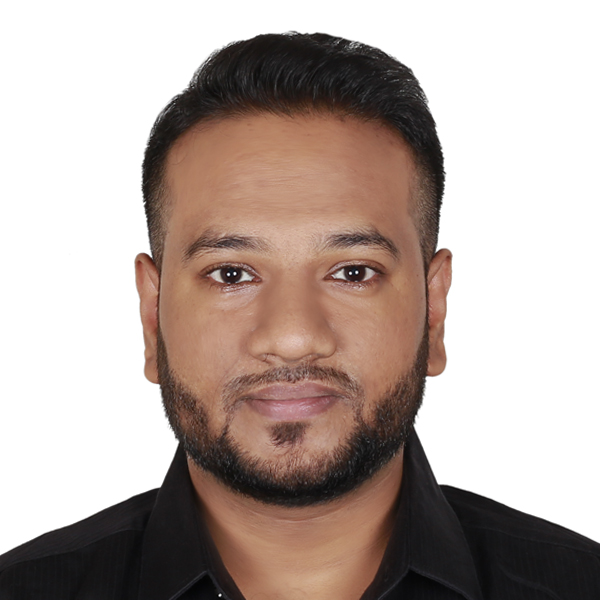
\includegraphics[width=4cm,clip,keepaspectratio]{profile.jpg}
        \end{minipage}
    \end{tabular}

%----------------------------------------------------------------------------------------
% TECHNICAL SKILLS SECTION
%----------------------------------------------------------------------------------------
    \begin{rSection}{Technical Skills}

        \textbf{Programming Languages:} Java, Kotlin, Python, Swift, C/C++, TypeScript, Shell Script\\
        \textbf{Databases:} MySQL, SQL Server, MongoDB, Firebase, Redis, InfluxDB\\
        \textbf{Cloud \& DevOps:} AWS, GCP, Nebius, Kaggle, Docker, Kubernetes (K3s, MicroK8s, Intel Tiber), Terraform, Ansible, CI/CD Pipelines, Grafana\\
        \textbf{AI Models:} Llama 3.2-3B Instruct, Llama 11B multimodal, Qwen 2.5 VL, Qwen 7B, Whisper, Kokoro TTS, ForwardTacotron+MelGAN, BAAI Embeddings, MobileSAM, Vision Transformer (ViT)\\
        \textbf{Network Technologies:} LTE/5G Network Deployment, IPsec VPN, TR-069, REST, MQTT, Google Protobuf, AMQP\\
        \textbf{Others:} Edge Computing, Kaggle, Mobile Application Development

    \end{rSection}


%----------------------------------------------------------------------------------------
% WORK EXPERIENCE SECTION
%----------------------------------------------------------------------------------------
    \begin{rSection}{Work Experience}

    {\bf Lead Sr. Software Engineer} \hfill July 2020 - Present\\
    NybSys Ltd, Dhaka, Bangladesh
    \begin{itemize}
        \itemsep -2pt
        \item Leading architecture, development, and deployment of \textbf{Sentra Gen-AI}, utilizing Kubernetes (K3s), Docker, Terraform, and CI/CD pipelines.
        \item Demonstrated Sentra Gen-AI (CPU/GPU) at \textbf{MWC Barcelona 2025} with global partners Intel (\href{https://www.youtube.com/watch?v=c-kq6M8Or5Q}{Intel Booth Demo}), Wind River (\href{https://www.youtube.com/watch?v=7MGbi-pOHqI}{Wind River Booth Demo}) and Lanner.
        \item \textbf{Sentra Gen-AI:} A versatile AI-driven platform providing secure, real-time encrypted socket communication across various platforms including Android, LMR, DMR, and Cisco IP phones. Sentra utilizes advanced Generative AI models (LLM, STT, TTS, Embeddings) for intelligent data processing, summarization, and communication. Engineered for seamless integration with diverse data sources like NMS, relational databases, and time-series databases, Sentra Gen-AI is suitable for multiple industries such as retail, hospitality, telecommunications, and beyond, enabling real-time insights, automated interactions, and data-driven decision-making.
        \item Developed and deployed other applications:
        \begin{itemize}
            \item \textbf{FaceNext (Android,AI,AWS,Python,DotNet)}: Attendance with face-liveness detection. \href{https://www.youtube.com/watch?v=uF53KBHzpME}{Youtube Link}
            \item \textbf{TillPay (Flutter)}: Mobile wallet app integrated with AWS SQS, SNS, REST APIs.
            \item \textbf{TillPay Merchant (Android)}: Built with AWS AppSync, Kotlin, Compose UI.
            \item \textbf{IG100 (Android)}: IoT controller app.
            \item \textbf{Truck Tracker (Android)}: Real-time location tracking, routing, and mapping.
            \item \textbf{DrinkWell Pump Operator \& Dealer (Flutter)}: Operational apps for DrinkWell personnel.
        \end{itemize}
        \item \textbf{Play Store:} \href{https://play.google.com/store/search?q=sentra&c=apps}{Sentra Client App}, \href{https://play.google.com/store/apps/details?id=com.nybsys.sentra.admin}{Sentra Admin App}
    \end{itemize}
    \vspace{4.0cm}
    {\bf Android Developer} \hfill Sept 2018 - Aug 2019\\
    W3Engineers Ltd, Khulna, Bangladesh
    \begin{itemize}
        \itemsep -2pt
        \item Led Android development and successfully published multiple apps on Evanto Market including:
        \begin{itemize}
            \item \href{https://codecanyon.net/item/videon-a-video-streaming-android-app-with-admin-panel/23466323}{Videon} (Streaming App)
            \item \href{https://codecanyon.net/item/bootic-an-android-ecommerce-app-with-admin-panel/22131989}{Bootic} (E-Commerce App)
            \item \href{https://codecanyon.net/item/qrcoba-a-qrbarcode-generator-and-scanner-android-app-with-admob/23127768}{QRcoba} (QR/Barcode Scanner)
        \end{itemize}
    \end{itemize}

    {\bf Android Coach} \hfill Oct 2019 - Oct 2020\\
    UY Systems Ltd, Dhaka, Bangladesh\\
    Trained professionals on advanced Android development, developed and maintained multiple Android applications for internal and Play Store deployment.

        {\bf Technical Trainer (Java \& Android)} \hfill Sept 2017 - Apr 2018\\
    Ernst \& Young LTD, Dhaka, Bangladesh\\
    Delivered Java and Android professional training across multiple educational institutes.

    \end{rSection}

%----------------------------------------------------------------------------------------
% EDUCATION SECTION
%----------------------------------------------------------------------------------------
    \begin{rSection}{Education}

        \textbf{M.Sc. in CSE}, Jahangirnagar University, Dhaka \hfill CGPA: 3.72 out of 4\\[1em]
        \textbf{B.Sc. in CSE}, BUBT, Dhaka \hfill CGPA: 3.01 out of 4\\[1em]
        \textbf{HSC}, FM International College, Dhaka \hfill GPA: 4.10 out of 5\\[1em]
        \textbf{SSC}, Paikgachha Govt. High School, Khulna \hfill GPA: 4.25 out of 5

    \end{rSection}

%----------------------------------------------------------------------------------------
% PERSONAL PROJECTS
%----------------------------------------------------------------------------------------
    \begin{rSection}{Personal Projects}

        \item \textbf{ICE Rover} (Hybrid Robot) – \href{https://www.youtube.com/watch?v=-xZL5QeMJOA}{YouTube Link}
        \item \textbf{Mars Rover Prototype} – \href{https://www.youtube.com/watch?v=Ezm-PA_P74U}{YouTube Link}
        \item \textbf{Quad Copter} – \href{https://www.youtube.com/watch?v=P7Kv3u3oT5Q}{YouTube Link}

    \end{rSection}

%----------------------------------------------------------------------------------------
% ACHIEVEMENTS SECTION
%----------------------------------------------------------------------------------------
    \begin{rSection}{Personal Achievements}
        \itemsep -2pt
        \item Champion, ROBO RUSH Project Exhibition (BUBT, 2018)
        \item UKURC Mars Rover Challenge Participant (UK, 2016)
        \item NASA App Challenge Certification (2016)
        \item 1st Runner-up, Intra-Intake Programming Contest (BUBT, 2013)
    \end{rSection}

%----------------------------------------------------------------------------------------
% PUBLICATIONS SECTION and Open Source Contribution
%----------------------------------------------------------------------------------------
    \begin{rSection}{Publications \& Open Source Contributions}
        \item \href{http://www.marspapers.org/paper/Sakib_2016.pdf}{\textbf{Low-Cost Design Approach and Evaluation of Mongolchari Mars Rover}}, presented at the 19th Annual International Mars Society Convention, 2016.

        \item \textbf{Open Source Contribution:} \href{https://github.com/GetStream/webrtc-in-jetpack-compose}{WebRTC in Jetpack Compose} (\href{https://github.com/GetStream/webrtc-in-jetpack-compose/pull/4}{Merged PR})\\
        Contributed Dockerization and streamlined the deployment process by containerizing the WebRTC signaling server, enhancing local testing and deployment ease.
    \end{rSection}


\end{document}
